\documentclass[a4paper]{article}
\usepackage{xgreek}
\usepackage{xunicode}
\usepackage{xltxtra}
\usepackage{setspace}
\usepackage{listings}
\usepackage{pdfpages}
\setlength{\parskip}{1ex}
\setlength{\topmargin}{0in}
\setlength{\oddsidemargin}{0in}
\setlength{\evensidemargin}{0in}
\setlength{\textheight}{9in}
\setlength{\textwidth}{6.25in}
\setmainfont[Mapping=tex-text]{DejaVu Sans}
\begin{document}
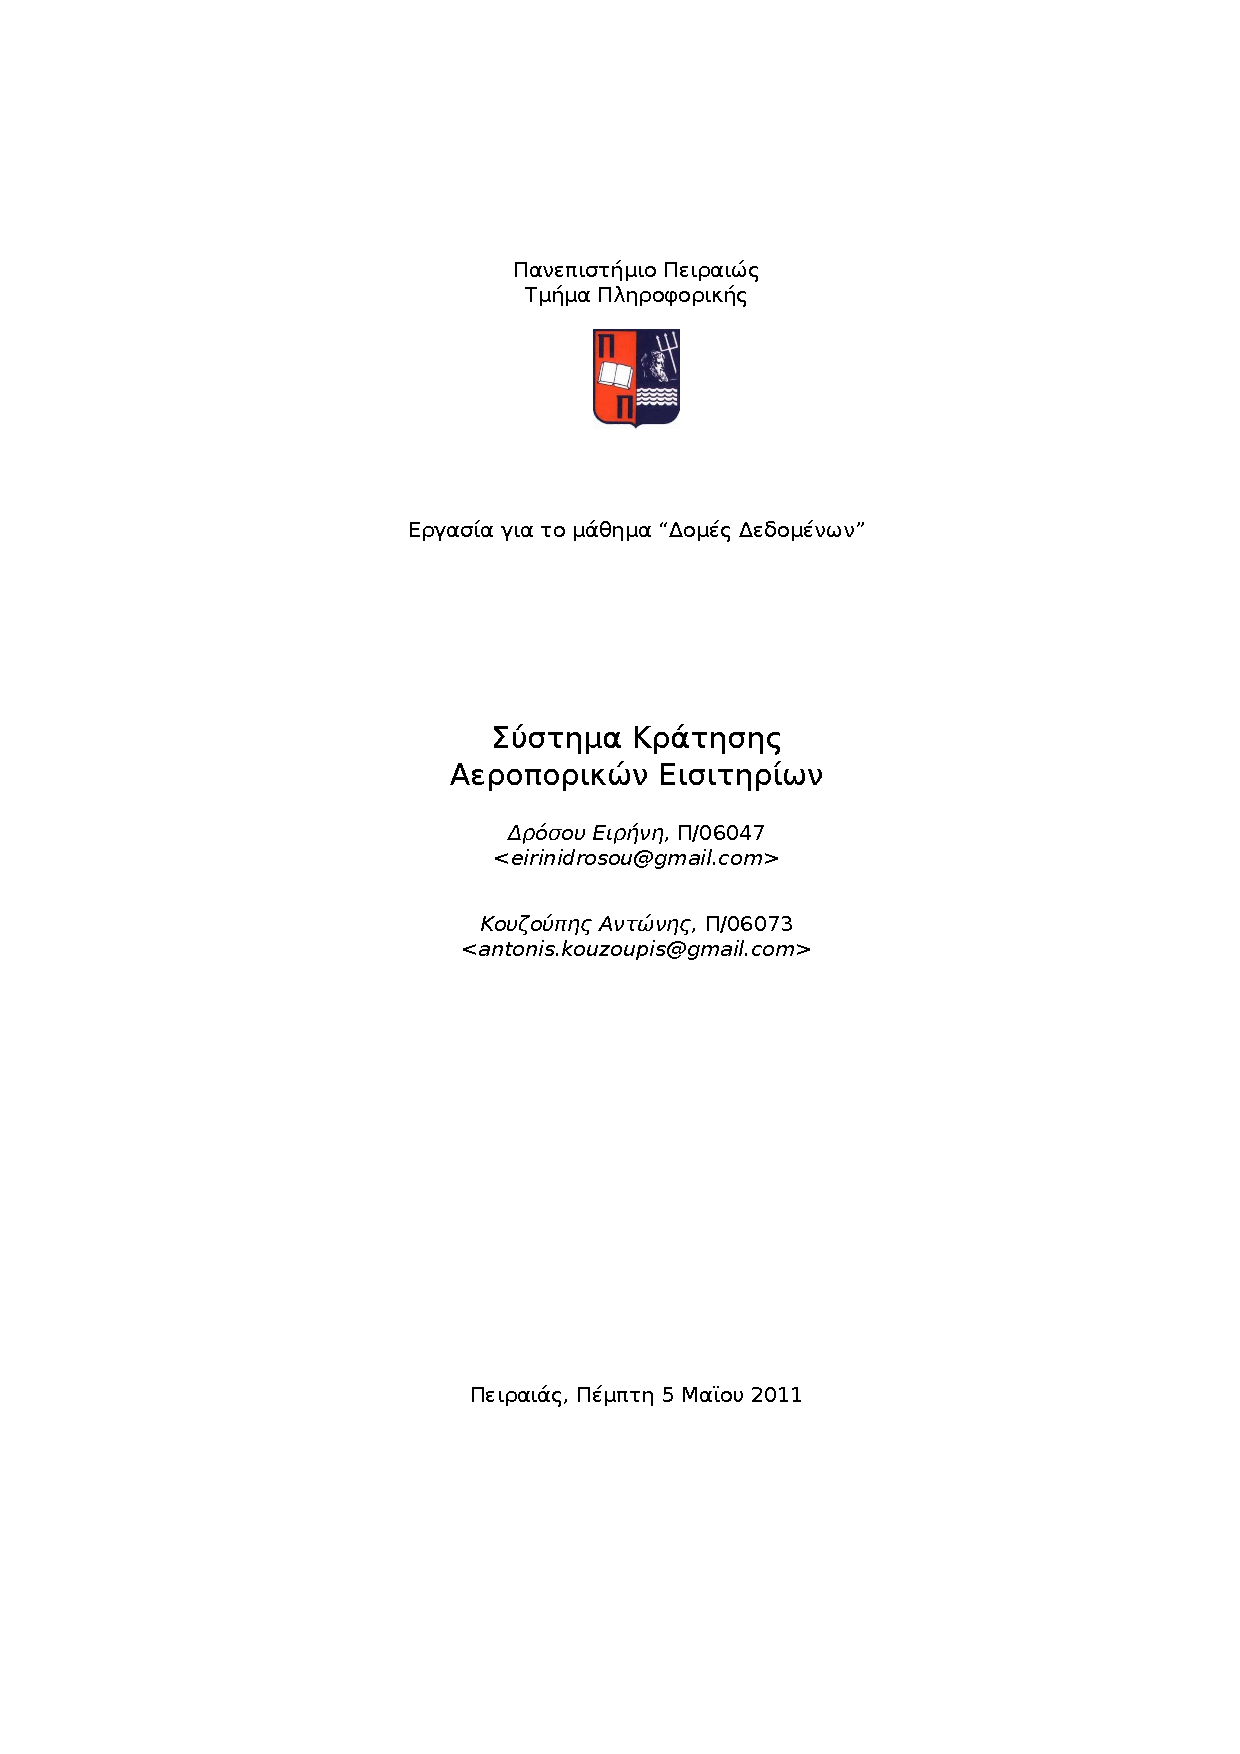
\includepdf[pages=-]{titlepage.pdf}
\tableofcontents
\newpage
\section{Εισαγωγή}
Η εφαρμογή υλοποιεί ένα απλοποιημένο σύστημα κράτησης αεροπορικών εισιτηρίων
Είναι γραμμένο στη γλώσσα προγραμματισμού Java. Οι δομές δεδομένων που
χρησιμοποιήθηκαν δεν είναι οι έτοιμες δομές που προσφέρει η γλώσσα. Η εφαρμογή
υποστηρίζει την προβολή, εισαγωγή και διαγραφή μιας πτήσης και τις αντίστοιχες
για τις κρατήσεις των επιβατών. Δεν χρησιμοποιεί κάποια τεχνολογία για
persistance καθώς δεν απαιτούνταν από την εργασία.

\section{Σχεδίαση}
Ο κώδικας της εφαρμογής είναι χωρισμένος σε τρία βασικά κομμάτια. Το κάθε
κομμάτι περιέχει κώδικα ``ανεξάρτητο'' από τα άλλα δύο. Παρόλα αυτά δεν είναι
κανένα αυτόνομο. Τα τρία directories--packages είναι τα \emph{business,
entities} και \emph{structures}. Το πρώτο package περιέχει όλο το business logic
της εφαρμογής. Δηλαδή περιέχει κλάσεις και μεθόδους που προσθέτει κάποιος μια
νέα πτήση, νέο επιβάτη κτλ. Το δεύτερο πακέτο αποτελείται από τις δύο οντότητες
της εφαρμογής, τους επιβάτες και τις πτήσεις. Οι κλάσεις αυτές είναι υπεύθυνες
για την αποθήκευση κρίσιμων πληροφοριών όπως Όνομα, Επίθετο κτλ για τους
επιβάτες και αριθμό πτήσης, ώρα αναχώρησης κτλ για τις πτήσεις. Το τρίτο και
τελευταίο κομμάτι έχει τις δομές δεδομένων που χρησιμοποιούμε στην εφαρμογή.
Συγκεκριμένα έχουμε υλοποιήσει μονά συνδεδεμένη λίστα, διπλά συνδεδεμένη λίστα
και ουρά αναμονής. Αναλυτικές πληροφορίες σχετικά με την υλοποίηση και την
εφαρμογή τους υπάρχουν στα σχόλια του κώδικα καθώς και στο Javadoc της
εφαρμογής.

\subsection{business package}
Το πακέτο αυτό περιέχει τις κλάσεις \emph{FlightsBusiness, Main,
PassengerBusiness} και \emph{Utilities}.

Η πρώτη κλάση έχει μεθόδους για τη δουλεία που γίνεται στη μεριά των πτήσεων.
Συγκεκριμένα διαχειρίζεται τη προ--φόρτωση κάποιων πτήσεων στο σύστημα, την
προβολή όλων των πτήσεων που είναι αποθηκευμένες στην εφαρμογή, την προσθήκη
νέων πτήσεων, τη διαγραφή πτήσεων, τη κράτηση πτήσεων από τους χρήστες, τον
έλεγχο της διαθεσιμότητας μιας πτήσης και τον έλεγχο των στοιχείων μιας
κράτησης.

Η δεύτερη κλάση αρχικοποιεί τις κατάλληλες δομές, τυπώνει το κεντρικό μενού και
αναλόγως την επιλογή καλεί τις κατάλληλες μεθόδους. Οι διαθέσιμες επιλογές του
χρήστη είναι η προβολή των διαθέσιμων πτήσεων, η προσθήκη μιας νέας πτήσης στο
σύστημα, η διαγραφή μιας πτήσης, η προσθήκη--κράτηση μιας κράτησης από τον
χρήστη, η προβολή όλων των επιβατών που έχουν καταχωρηθεί στην εφαρμογή, η
διαγραφή ενός επιβάτη και της κράτησής του και η έξοδος από την εφαρμογή.

Τρίτη κλάση είναι η \emph{PassengerBusiness} η όποια είναι υπεύθυνη για τις
λειτουργίες που αφορούν τους χρήστες. Χρησιμοποιείται για να εκτύπωση όλων των
επιβατών στο σύστημα, την εκτύπωση των κατάλληλων ``ερωτήσεων'' κατά την
εισαγωγή ενός νέου επιβάτη, για την εισαγωγή ενός νέου επιβάτη--κράτησης και για
την διαγραφή μιας κράτησης.

Τέλος η κλάση \emph{Utilities} περιέχει δύο βοηθητικές μεθόδους. Η πρώτη είναι
μία υλοποίηση της συνάρτησης κατακερματισμού md5 και η άλλη είναι η μετατροπή
μιας συμβολοσειράς σε δεκαεξαδική μορφή. Η τελευταία χρησιμοποιείται από την
μέθοδο που υλοποιεί το md5 hash.

\subsection{entities package}
Το πακέτο \emph{entities} περιέχει τις κλάσεις \emph{Flight} και
\emph{Passenger}.

Η κλάση \emph{Flight} είναι υπεύθυνη για την αποθήκευση όλων των στοιχείων
μιας πτήσης. Συγκεκριμένα τα στοιχεία που κρατάει είναι ο κωδικός πτήσης, την
αφετηρία, τον προορισμό, την ώρα αναχώρησης, την ώρα άφιξης, τη τιμή των
εισιτηρίων, τον τύπο του αεροσκάφους, των συνολικό αριθμό θέσεων στο αεροπλάνο,
τις διαθέσιμες θέσεις στο αεροπλάνο, τους επιβάτες που έχουν κάνει κράτηση για
τη συγκεκριμένη πτήση και υπάρχει θέση στο αεροπλάνο και τους επιβάτες οι οποίοι
έχουν κάνει κράτηση για τη συγκεκριμένη πτήση αλλά δεν υπάρχουν διαθέσιμες
θέσεις οπότε μπαίνουν σε λίστα αναμονής. Οι μέθοδοι που υπάρχουν είναι για να
θέτουμε μία νέα τιμή στις παραπάνω μεταβλητές και για να παίρνουμε τις τιμές των
παραπάνω μεταβλητών (getters \& setters). Επίσης υπάρχει και μία μέθοδος για την
εκτύπωση όλων των παραπάνω λεπτομερειών.

Η κλάση αυτή είναι υπεύθυνη για την αποθήκευση των λεπτομερειών ενός χρήστη
και της κράτησής του. Τα στοιχεία που κρατάει είναι το επίθετο, το όνομα, τον
αριθμό ταυτότητας, την εθνικότητα, τη διεύθυνση, το τηλέφωνο, το μοναδικό αριθμό
κράτησης του χρήστη, την κατάσταση της κράτησής του και μία λίστα με τους
κωδικούς πτήσης των δρομολογίων που έχει κάνει κράτηση. Οι μέθοδοι που υπάρχουν
στη κλάση αυτή είναι για να ορίζουμε μία νέα τιμή στα παραπάνω στοιχεία και για
να παίρνουμε την υπάρχουσα τιμή τους. Υπάρχει και μία μέθοδος για την εκτύπωση
όλων των παραπάνω στοιχείων.

\subsection{structures package}
Το πακέτο αυτό περιέχει τις κλάσεις \emph{DoublyLinkedList, FifoQueue} και
\emph{SimplyLinkedList}.

Η κλάση \emph{DoublyLinkedList} υλοποιεί τη διπλά συνδεδεμένη λίστα που
χρησιμοποιείται στην εφαρμογή. Χρησιμοποιεί τα Generics της Java για τον
προσδιορισμό του τύπου των στοιχείων που θα κρατάει. Αποτελείται από δύο
κλάσεις, την \emph{DNode} που κρατάει τις πληροφορίες για κάθε κόμβο όπως την
τιμή του κόμβου, τον επόμενο και τον προηγούμενο κόμβο καθώς και κάποιες
μεθόδους για την προσπέλαση των παραπάνω στοιχείων. Η δεύτερη κλάση είναι η
\emph{DoublyLinkedList} που υλοποιεί κάποιες λειτουργίες της διπλά συνδεδεμένης
λίστας όπως την διαγραφή ενός κόμβου ενώ παίρνουμε και την τιμή του, την
προσθήκη σε κάποια συγκεκριμένη θέση στη λίστα, την προσθήκη ενός κόμβου στην
αρχή, στο τέλος, μία μέθοδος για να παίρνουμε το μέγεθος της λίστας, μία για να
ξέρουμε αν η λίστα είναι άδεια και μία για να τυπώνουμε όλα τους κόμβους της
λίστας.

Η κλάση \emph{FifoQueue} υλοποιεί μία FIFO (First In First Out) ουρά αναμονής
βασισμένη σε μία απλά συνδεδεμένη λίστα. Χρησιμοποιεί επίσης τα Generics της
Java. Έχει δύο κλάσεις, η μία είναι η \emph{QNode} όπου κρατάει τα στοιχεία ενός
κόμβου όπως την τιμή του κόμβου και τον επόμενο κόμβο. Επίσης έχει κάποιες
μεθόδους για την προσπέλαση των στοιχείων αυτών. Τέλος η κλάση \emph{FifoQueue}
περιέχει μεθόδους για τις βασικές λειτουργίες της ουράς όπως είναι η εισαγωγή
στο τέλος, η εξαγωγή από την αρχή, η διαγραφή ενός στοιχείου στο ενδιάμεσο της
ουράς, μέθοδος για να παίρνουμε το μέγεθος της ουράς, για να βλέπουμε αν είναι
άδεια και μία μέθοδος για να τυπώνει τις τιμές των κόμβων της ουράς αναμονής.

Τέλος η κλάση \emph{SimplyLinkedList} υλοποιεί μία μονά συνδεδεμένη λίστα που
επίσης χρησιμοποιεί Generics. Αποτελείται και αυτή από δύο κλάσεις, η μία είναι η
\emph{SNode} που κρατάει διάφορες πληροφορίες για ένα κόμβο όπως τη τιμή του
κόμβου και τον επόμενο κόμβο. Έχει επίσης κάποιες μεθόδους για την προσπέλαση
των στοιχείων αυτών. Η κλάση \emph{SimplyLinkedList} υλοποιεί κάποιες
λειτουργίες της μονά συνδεδεμένης λίστας όπως την προσθήκη ενός κόμβου είτε στην
αρχή, είτε στο τέλος είτε κάπου ενδιάμεσα, τη διαγραφή ενός κόμβου, μέθοδο για
την παίρνουμε το μέγεθος της λίστας, μέθοδο για να βλέπουμε αν η λίστα είναι
άδεια και μία μέθοδο που τυπώνει τις τιμές όλων των κόμβων της λίστας.

\subsection{Δομή Εφαρμογής}
Οι δύο οντότητες της εφαρμογής είναι οι πτήσεις και οι επιβάτες--κρατήσεις. Τα
χαρακτηριστικά στοιχεία των πτήσεων κρατούνται στην κλάση \emph{Flight}, δηλαδή
κάθε πτήση είναι ένα instance της κλάσης αυτής. Κάθε πτήση, εκτός από τα
στοιχεία που αναφέρονται παραπάνω, έχει μία λίστα μονά συνδεδεμένη με τους
κωδικούς κράτησης και μία ουρά αναμονής με τους κωδικούς κράτησης που ναι μεν
έχουν κάνει κράτηση αλλά επειδή δεν υπήρχε διαθέσιμη θέση, μπήκαν σε ουρά
αναμονής. Όλες οι πτήσεις, δηλαδή τα instances της κλάσης Flight κρατούνται σε
μία διπλά συνδεδεμένη λίστα.

Για κάθε επιβάτη που κάνει επιτυχώς μία κράτηση, κρατούνται τα προσωπικά του
στοιχεία καθώς και μία λίστα με τους κωδικούς πτήσεων που έχει κρατήσει θέση. Η
λίστα αυτή είναι μία μονά συνδεδεμένη λίστα. Επίσης για κάθε επιβάτη--κράτηση
δημιουργείται ένα μοναδικό ``κλειδί''. Όλοι οι επιβάτες, δηλαδή instances της
κλάσης \emph{Passenger} κρατούνται σε μία διπλά συνδεδεμένη λίστα.

\section{Επεξήγηση Λειτουργίας}
Για να τρέξει η εφαρμογή χρειάζεται το runtime enviroment της Java. Τα binaries
είναι αρχειοθετημένα σε ένα archive τύπου jar. Οπότε για να εκτελέσουμε την
εφαρμογή αρκεί να πάμε στον κατάλογο που βρίσκεται το αρχείο
\emph{DataStruct.jar} και εκτελούμε \emph{java -jar DataStruct.jar}.
Εμφανίζεται ένα μενού με τις διαθέσιμες λειτουργίες. Το μενού θα εμφανίζεται
έπειτα από κάθε ενέργεια μέχρι να δώσουμε την επιλογή εξόδου.

Επίσης η κλάση \emph{Main} δημιουργεί τις λίστες με τους επιβάτες και τις
πτήσεις ώστε να είναι διαθέσιμες στην εφαρμογή.

\subsection{View Available Flights}
Με την επιλογή αυτή, τυπώνεται όλη η λίστα με τις πτήσεις που είναι
καταχωρημένες στην εφαρμογή. Συγκεκριμένα επιλέγοντας την πρώτη επιλογή,
καλείται η μέθοδος \emph{listFlights} της κλάσης \emph{FlightsBusiness}. Αυτή με
τη σειρά της καλεί την μέθοδο \emph{toString} της κλάσης \emph{DoublyLinkedList}
όπου είναι η λίστα που κρατάει τις πτήσεις. Τέλος από αυτή καλείται η
\emph{toString} της κλάσης \emph{Flight} που τυπώνει τα χαρακτηριστικά μιας
πτήσης.

\subsection{Add Flight}
Με την δεύτερη επιλογή μπορούμε να προσθέσουμε πτήσεις στο σύστημα. Καλείται η
μέθοδος \emph{addFlight} της κλάσης \emph{FlightsBusiness} όπου ρωτάει τον
χρήστη ποια θα είναι τα χαρακτηριστικά της νέας πτήσης. Ο κωδικός πτήσης μπορεί
να είναι είτε κεφαλαία είτε πεζά. Για την καταχώρηση της
ημερομηνίας αναχώρησης και άφιξης χρησιμοποιείται η κλάση \emph{Gregorian
Calendar}, η κλάση \emph{Date} και η μέθοδος \emph{getTime }της Java που 
μετατρέπουν την ημερομηνία σε milliseconds από το EPOCH. Έπειτα δημιουργείται
ένα νέο αντικείμενο τύπου \emph{Flight} με τις παραπάνω τιμές και το βάζουμε στη
λίστα με τις υπόλοιπες διαθέσιμες πτήσεις μέσω της μεθόδου \emph{addTail} της
κλάσης \emph{DoublyLinkedList}.

\subsection{Remove Flight}
Με την επιλογή αυτή μπορούμε να διαγράψουμε μία διαθέσιμη πτήση. Επιλέγοντάς
την, καλείται η μέθοδος \emph{removeFlight} της κλάσης \emph{FlightBusiness}.
Μας ρωτάει τον κωδικό πτήσης και ψάχνει για το συγκεκριμένο αντικείμενο στη
λίστα με τις διαθέσιμες πτήσεις. Αφού το βρει, το διαγράφει.

\subsection{Add Passenger}
Η επιλογή Add Passenger προσθέτει έναν επιβάτη και μία κράτηση στο σύστημα.
Αρχικά καλείται η μέθοδος \emph{askPassenger} της κλάσης
\emph{PassengerBusiness} όπου ρωτάει τον χρήστη για τα προσωπικά του στοιχεία
και τους κωδικούς πτήσεων των πτώσεων που θέλει να κλείσει. Οι κωδικοί πτήσεων 
μπορεί να είναι είτε κεφαλαία είτε πεζά. Στη συνέχεια καλείται
η μέθοδος \emph{validateFlights} της κλάσης \emph{FlightsBusiness} όπου
ελέγχει αν μία κράτηση είναι έγκυρη Αν ο χρήστης έχει κάνει κράτηση μιας πτήσης
χωρίς ενδιάμεση στάση τότε προφανώς είναι έγκυρη Σε αντίθετη περίπτωση θα
πρέπει ο προορισμός της πρώτης να είναι ίδιος με την αφετηρία της επόμενης και η
ώρα άφιξης της πρώτης να είναι πριν την ημερομηνία αναχώρησης της επόμενης.
Αυτός ο έλεγχος γίνεται για όσες πτήσεις έχει δώσει ο χρήστης. Αν οι κράτηση
βγει άκυρη τότε εκτυπώνεται κατάλληλο μήνυμα και ο χρήστης βγαίνει πάλι στο
κεντρικό μενού όπου μπορεί να ξαναπροσπαθήσει.

Σε αντίθετη περίπτωση, καλείται η μέθοδος \emph{addPassenger} της κλάσης
\emph{PassengerBusiness}. Η μέθοδος αυτή προσθέτει στη λίστα με τους επιβάτες
τον νέο επιβάτη. Επίσης δημιουργεί ένα μοναδικό κλειδί για αυτή την κράτηση ώστε
να μπορεί αργότερα να τη διαγράψει, αλλά βοηθάει και στην λειτουργία της
εφαρμογής. Το κλειδί είναι το md5sum του αριθμού ταυτότητας του χρήστη και των
κωδικών πτήσεων που έχει κάνει κράτηση. Ακολουθεί η μέθοδος \emph{checkAvailability} της κλάσης
\emph{FlightsBusiness} με όρισμα το αντικείμενο μιας πτήσης που αντιστοιχεί στον
κωδικό πτήσης που έχει δώσει ο χρήστης. Με αυτό τον τρόπο ελέγχεται αν σε κάθε
πτήση υπάρχει διαθέσιμη θέση σε κάθε πτήση. Αν έστω και σε μία πτήση δεν υπάρχει
διαθέσιμη θέση τότε ο χρήστης μπαίνει στις ουρές αναμονής όλων των πτήσεων. Στη
συνέχει καλείται η \emph{bookFlight} της κλάσης \emph{FlightsBusiness} με όρισμα
τους κωδικούς πτήσεων που έχει δώσει ο χρήστης, το μοναδικό κλειδί της κράτησης
και μία επιλογή με διαφορετική τιμή αναλόγως την διαθεσιμότητα των θέσεων. Όπως
αναφέραμε να παραπάνω, αν υπάρχουν διαθέσιμες θέσεις σε όλες τις πτήσεις, τότε ο
κωδικός της κράτησης αποθηκεύεται στη λίστα επιβίβασης κάθε πτήσης και
μειώνονται οι διαθέσιμες θέσεις. Αν δεν υπάρχουν διαθέσιμες θέσεις τουλάχιστον
σε μία πτήση, τότε ο κωδικός της κράτησης αποθηκεύεται στις ουρές αναμονής κάθε
πτήσης. Τελειώνοντας μέσω της μεθόδου \emph{setStatus} της κλάσης
\emph{Passenger} θέτουμε την διαθεσιμότητα της κράτησης.

\subsection{List Passengers}
Με την επιλογή List Passengers μπορούμε να δούμε όλους τους επιβάτες που έχουν
κάνει κράτηση μέσω της εφαρμογής. Με την επιλογή αυτή καλείται η μέθοδος
\emph{listPassengers} της κλάσης \emph{PassengerBusiness}. Αυτή καλεί την μέθοδο
\emph{toString} της κλάσης \emph{DoublyLinkedList} όπου τυπώνει την τιμή κάθε
αντικειμένου που είναι αποθηκευμένο στη λίστα. Αυτή με τη σειρά της καλεί την
μέθοδο \emph{toString} της κλάσης \emph{Passenger} όπου τελικά τυπώνει τα
χαρακτηριστικά μιας κράτησης.

\subsection{Delete Passenger}
Με αυτή την επιλογή ένας επιβάτης μπορεί να διαγράψει την κράτηση που έχει
κάνει. Μία κράτηση μπορεί να βρίσκεται σε δύο δυνατές καταστάσεις. Μπορεί να
βρίσκεται στις λίστες αναμονής των πτήσεων ή μπορεί να βρίσκεται στις λίστες
επιβίβασης των πτήσεων. Αναλόγως την κατάσταση, ακολουθείται διαφορετική λογική
και διαδικασία κατά την διαγραφή.

Αν μία κράτηση βρίσκεται σε κατάσταση pending, δηλαδή ο επιβάτες είναι στις
ουρές αναμονής των πτήσεων του, τότε αρκεί απλά να τον διαγράψουμε από τις
παραπάνω λίστες αναμονής. Οπότε για κάποιο επιβάτη σε αυτή την κατηγορία,
παίρνουμε τη λίστα \emph{bookedFlightsList} που κρατάει τις πτήσεις που έχει
κάνει κράτηση ο χρήστης και διαγράφουμε από αυτές τον κωδικό κράτησης του (του
επιβάτη). Τέλος διαγράφουμε τον επιβάτη και από τη λίστα με τους επιβάτες.

Αν μία κράτηση βρίσκεται σε κατάσταση boarding, δηλαδή ο επιβάτης βρίσκεται στις
λίστες επιβίβασης των πτήσεων που έχει κάνει κράτηση, τότε ακολουθείται
διαφορετική διαδικασία. Η λογική είναι ότι όταν διαγράφεται ένας χρήστης από μία
λίστα επιβίβασης, κοιτάμε στην ουρά αναμονής της αντίστοιχης πτήσης, αν υπάρχει
επιβάτης του οποίου η κατάσταση κράτησης μπορεί να γίνει boarding έπειτα από τη
διαγραφή του πρώτου, δηλαδή σε όλες τις πτήσεις που έχει κάνει κράτηση υπάρχουν
διαθέσιμες θέσεις, τότε τον βάζουμε στις λίστες επιβίβασης των πτήσεων του. Αν
δεν βρεθεί τέτοιος επιβάτης μένει κενή μία θέση στην πτήση. Επομένως από τον
επιβάτη προς διαγραφή, παίρνουμε τη λίστα με τους κωδικούς πτήσεών του και
παίρνουμε την πρώτη πτήση. Από την πρώτη πτήση παίρνουμε τη λίστα αναμονής της.
Για κάθε έναν επιβάτη στη λίστα αναμονής ελέγχουμε αν κάθε μία πτήση του έχει
διαθέσιμες θέσεις έπειτα από τη διαγραφή του πρώτου επιβάτη. Αν βρεθεί τέτοιος
επιβάτης, τον διαγράφουμε από τις ουρές αναμονής των πτήσεων που έχει κάνει
κράτηση και τον τοποθετούμε στις λίστες επιβίβασης αυτών των πτήσεων. Τελικά
διαγράφουμε τον χρήστη και από τη λίστα με τους επιβάτες.
\subsection{Exit}
Με την επιλογή αυτή βγαίνουμε από την εφαρμογή. Επειδή δεν έχει υλοποιηθεί
κάποιος τρόπος για μόνιμη αποθήκευση, έπειτα από την έξοδο, όποια καταχώρηση
είχε γίνει χάνεται.
\end{document}
